\chapter{Entropia e Informazione di Shannon}

\section{Informazione di Shannon}
L'\textbf{Informazione di Shannon} associata a un valore $x \in \mathcal A_X$ di una variabile aleatoria $X$ è definita come:
$$
h(x) = \log_{2}\frac{1}{P[x]}
$$
e si misura in \textbf{bit}.

\section{Entropia di una variabile aleatoria}
L'entropia (o incertezza) di una variabile aleatoria $X$ è definita come il valore atteso dell'informazione di Shannon.
$$
H(X) = \sum_{x\in A_X}P[x]\log\frac{1}{P[x]} \hspace{0.5cm} 0\le H(X)\le \log \left| A_X \right| 
$$

e si misura in \textbf{bit}. Inoltre se $P[x] = 0$, accetteremo che $P[x] \log_{2} \frac{1}{P[x]} = 0$, ossia, un evento impossibile trasporta informazione nulla.

\subsection{Proprietà dell'entropia}
L'entropia gode di alcune proprietà fondamentali:

\begin{enumerate}
	\item \textbf{Non negatività}: L'entropia di una variabile aleatoria non può essere negativa. 
	$$
	H(X) \geq 0 
	$$
	\textbf{Dimostrazione}: Si dimostra notando che nella formula dell'entropia:
	$$
	H(X) = \sum_{x\in A_X} P(x)\log_{2}\frac{1}{P(x)}
	$$
	che $\log_{2}\frac{1}{P(x)} \geq 0$ in quanto $0 \leq P(x) \leq 1$
	
	\item \textbf{Entropia Massima}: L'entropia di una variabile aleatoria è \textbf{massima} quando abbiamo una distribuzione \textbf{uniforme}, ed è:
	$$
	H(X) \leq \log_{2}(|A_x|)
	$$
	
	\item \textbf{Ridondanza}: La ridondanza misura la \textbf{differenza} tra $H(X)$ e il suo valore massimo possibile, ovvero $\log_{2}(|A_x|)$.
	
	\item \textbf{Entropia Congiunta}: L'entropia di due variabili aleatorie $X$ ed $Y$ (dipendenti tra loro) è:
	$$
	H(X,Y) = \sum_{x\in A_X,y\in A_Y}P(x,y) \log\frac{1}{P(x,y)}
	$$
	
	\item \textbf{Entropia tra VA indipendenti}: L'entropia tra due variabili aleatorie \textbf{indipendenti} consiste nella somma delle entropie delle singole VA:
	$$
	H(X,Y) = H(X)+H(Y)
	$$
	
	\item \textbf{Entropia Condizionata}: L'entropia condizionata di due variabili aleatorie $X$ ed $Y$ descrive quanti bit di informazione sono \textbf{necessari}, in media, per descrivere $X$ conoscendo l'informazione acquisita da $Y$, e si misura così:
	$$
	H(X|Y) = \sum_{x\in A_X,y\in A_Y}P[x,y] \log\frac{1}{P[x|y]}
	$$
\end{enumerate}

\subsection{Regola della Catena per l'entropia} 
La Regola della Catena misura l'entropia totale su due variabili aleatorie $X$ e $Y$, data dall'entropia di $X$ più l'entropia di $Y$ conoscendo quella di $X$:
\begin{equation}
	H(X,Y) = H(X) + H(Y|X)
\end{equation}

\subsubsection{Dimostrazione della Regola della Catena}
Si dimostra partendo dalla formula dell'\textbf{Entropia Congiunta}:
$$
H(X,Y) = \sum_x\sum_yP[x,y]\log_{2}\frac{1}{P[x,y]}=\sum_x\sum_y P[x,y]\log_{2}\frac{1}{P[y|x]P[x]}=
$$
$$
\sum_x\sum_yP[x,y](\log_{2}\frac{1}{P[y|x]} ) + \log_{2} \frac{1}{P[x]} = \sum_{x,y}P[x,y] \log_{2}\frac{1}{P[y|x]} + \sum_{x,y}P[x,y]\log_{2}\frac{1}{P[x]}
$$
$$
H(X,Y) = \sum_x\sum_yP[x,y]\log\frac{1}{P[x,y]}=\sum_x\sum_y P[x,y]\log\frac{1}{P[y|x]P[x]}=
$$
$$\sum_x\sum_yP[x,y](\log\frac{1}{P[y|x]})+\log\frac{1}{P[x]} =
\sum_{x,y}P[x,y]\log\frac{1}{P[y|x]}+\sum_{x,y}P[x,y]\log\frac{1}{P[x]}
$$
$$
H(X,Y) = \sum_x\sum_yP[x,y]\log\frac{1}{P[x,y]} = \sum_x\sum_y P[x,y]\log\frac{1}{P[y|x]P[x]} =
$$
$$
\sum_x\sum_yP[x,y](\log\frac{1}{P[y|x]}) + \log\frac{1}{P[x]} =
\sum_{x,y}P[x,y]\log\frac{1}{P[y|x]} + \sum_{x,y}P[x,y]\log\frac{1}{P[x]}
$$

Adesso notiamo che:
$$
\sum_{x,y} P[x,y]\log\frac{1}{P[y|x]} = H(Y|X) \quad \text{e} \quad \sum_{x,y}P[x,y]\log\frac{1}{P[x]} = H(x)
$$
per cui:
$$
H(X,Y) = H(Y|X)+H(X)
$$

\newpage
\subsubsection{Esempio N.1 - Entropia}
Supponiamo di avere una variabile aleatoria $X$, con:
\begin{itemize}
	\item $A_X = \{a,b,c,d,e,f,g,h\}$
	\item $Pr_x = \{\frac{1}{4},\frac{1}{8},\frac{1}{8},\frac{1}{4},\frac{1}{32},\frac{1}{32},\frac{1}{16},\frac{1}{8}\}$
\end{itemize}
dove:
$$
Pr[X=a] = \frac{1}{4}\quad;\quad Pr[X=b] = \frac{1}{8}\quad;\quad Pr[X=c] = \frac{1}{8} \quad; \quad \text{etc...}
$$
Calcolare l'entropia di $X$

Per calcolare l'entropia di $X$ applico la formula dell'entropia:
$$
H(X) = \sum_{x\in A_X} Pr[X = x] \log_{2} \frac{1}{Pr[X = x]}
$$
Quindi:
$$
H(X) = \frac{1}{4}\cdot\log_{2}4 + \frac{1}{8}\cdot\log_{2}8 + \frac{1}{8}\cdot\log_{2}8 + \frac{1}{4}\cdot\log_{2}4 + \frac{1}{32}\cdot\log_{2}32 + \frac{1}{32}\cdot\log_{2}32 + \frac{1}{16}\cdot\log_{2}16 + \frac{1}{8}\cdot\log_{2}8 =
$$
$$
= \frac{1}{2}\cdot\log_{2}4 + \frac{3}{8}\cdot\log_{2}8 + \frac{2}{32}\cdot\log_{2}32 + \frac{1}{16}\cdot\log_{2}16 = \frac{1}{2}\cdot2 + \frac{3}{8}\cdot3 + \frac{1}{16}\cdot5 + \frac{1}{16} =
$$
$$
= 1 + \frac{9}{8} + \frac{9}{16} = \frac{16 + 18 + 9}{16} = \frac{43}{16} \approx 2,69 \approx 2,7
$$

\subsubsection{Esempio N.2 - Entropia con $p$ uniforme}
Supponiamo di avere una variabile aleatoria $X$, con $A_X = \{a,b,c,d,e,f,g,h\}$ dove $$\forall x \in A_X \Rightarrow Pr[X = x] = \frac{1}{8}$$

Calcolare l'entropia di X

Uso nuovamente la formula dell'entropia:
$$
H(X) = \sum_{x\in A_X} Pr[X = x] \log_{2} \frac{1}{Pr[X = x]} =
8 \cdot \frac{1}{8} \cdot \log_{2}8 = 3
$$
Notiamo inoltre che essendo una distribuzione \textbf{uniforme}, l'entropia calcolata è \textbf{massima}.

\subsubsection{Esempio N.3 - Entropia con evento certo}
Supponiamo di avere una variabile aleatoria $X$, con:
\begin{itemize}
	\item $A_X = \{a,b,c,d,e,f,g,h\}$
	\item $Pr_x = \{1,0,0,0,0,0,0,0\}$
\end{itemize}
dove:
$$
Pr[X=a] = 1\quad;\quad Pr[X=b] = 0\quad;\quad Pr[X=c] = 0 \quad; \quad \text{etc...}
$$
Calcolare l'entropia di X

Uso nuovamente la formula dell'entropia:
$$
H(X) = \sum_{x\in A_X} Pr[X = x] \log_{2} \frac{1}{Pr[X = x]} =
1 \cdot \log_{2}1 = 0
$$

Notiamo che l'entropia in un evento certo è 0, in quanto non può esservi incertezza in un evento sicuro.
\newpage

\section{Entropia relativa}
Prima di discutere l'entropia relativa, andremo a introdurre dei concetti utili per le nostre dimostrazioni.


\subsection{Funzioni convesse e disuguaglianza di Jensen}

\paragraph{Funzioni Convesse}
Una funzione $f(x)$ è \textbf{convessa} in un intervallo $(a,b)$ se ogni \textit{corda} (segmento) della funzione si trova \textbf{sopra} la funzione, ovvero se $\forall x_1, x_2 \in (a,b)$ e $0 \leq \lambda \leq 1$ abbiamo:

\begin{equation}
	f(\lambda x_1  + (1-\lambda)x_2) \leq \lambda f(x_1) + (1-\lambda) f(x_2)
\end{equation}

Una funzione $f(x)$ è \textbf{strettamente convessa} se $\forall x_1, x_2 \in (a,b)$ abbiamo $\lambda = 0$ o $\lambda = 1$

Esempi di funzioni \textbf{strettamente convesse} sono:
\begin{itemize}
	\item $x^2,\ e^x\ \text{e}\ e^{-x}$ per ogni $x$;
	\item $\log(1/x)$ e $x \log x$ per ogni $x>0$
\end{itemize}

\paragraph{Diseguaglianza di Jensen}
Se una funzione $f(x)$ è una funzione \textbf{convessa} e $x$ è una variabile aleatoria, allora:
\begin{equation}
	E[f(X)] \geq f(E[X])
\end{equation}
Inoltre se la funzione è \textbf{strettamente convessa} e $E[f(X)] = f(E[X])$ allora la variabile aleatoria $x$ è una costante.\\ La diseguaglianza di Jensen può essere riscritta se la funzione è concava, invertendo il senso.

\textbf{Dimostrazione}:

Dimostriamola per induzione su $\left| A_x \right|$:
\begin{itemize}
	\item \textbf{Caso base}: Con $\left|A_x\right|=2 \hspace{0.5cm} e \hspace{0.5cm} x_1,x_2 \hspace{0.3cm} con \hspace{0.3cm} p_1,p_2=1-p_1$ allora: $$E(f(X))=p_1f(x_1)+p_2(fx_2)=p_1(fx_1)+(1-p_1)f(x)\ge f(p_1x_1+(1-p_1)x_2)=f(E(X))$$
	
	\item \textbf{Passo Induttivo}: Essendo la tesi vera per $\left| A_x \right| = k$, la dimostriamo per $k+1$:
	$$E[f(X)] = \sum^{k+1}_{i=1}p_if(x_i)=p_{k+1}f(x_{k+1})+\sum^k_{i=1}p_if(x_i) = p_{k+1}f(x_{k+1})+(1-p_{k+1})\sum^k_{i=1}\frac{p_i}{1-p_{k+1}}f(x_i)$$
	Applicando Jensen:
	$$\ge p_{k+1}f(x_{k+1})+(1-p_{k+1})f\left(\sum^k_{i=1}\frac{p_i}{1-p_{k+1}}x_i\right)$$
	per la concavità di $f$:
	$$\ge f\left(p_{k+1}x_{k+1}+(1-p_{k+1})\sum^k_{i=1}\frac{p_i}{1-p_{k+1}}x_i\right) = f\left(p_{k+1}x_{k+1}+\sum^k_{i=1}p_ix_i\right) = f\left( \sum^{k+1}_{i=1}x_ip_i\right)=f(E[X])$$
\end{itemize}

\newpage
\subsection{Entropia Relativa (o Divergenza di Kullback-Leibler)}
L'entropia relativa tra due distribuzioni di probabilità $P(x)$ e $Q(x)$ definite nello stesso insieme $A_X$ misura l'inefficienza di assumere che la corretta distribuzione sia $Q$ quando invece è $P$, ed è:
\begin{equation}
	\begin{aligned}
		D_{KL}(P||Q)=\sum_{x\in A_x}P(x)\log\frac{P(x)}{Q(x)}
	\end{aligned}
\end{equation}
È importante notare che l'Entropia Relativa \textbf{non è simmetrica}, quindi:
$$
D_{KL}(P||Q) \neq D_{KL}(Q||P)
$$

L'entropia relativa soddisfa la \textbf{Diseguaglianza di Gibbs}:
\begin{equation}
	D_{KL}(P||Q) \geq 0
\end{equation}
ossia è sempre non negativa. $D_{KL}(P||Q) = 0$ se e solo se $P = Q$

\paragraph{Dimostrazione della Diseguaglianza di Gibbs}
$$
-D_{KL}=-\sum_{x\in A_X}P(x)\log\frac{P(x)}{Q(x)} = \sum_{x\in A_X}P(x)\log\frac{Q(x)}{P(x)}
$$
essendo il logaritmo una funzione concava applichiamo la \textbf{disuguaglianza di Jensen}:
$$
\le\log\sum_{x\in A_X} P(X)\frac{Q(X)}{P(X)} = \log\sum_{x\in A_X} Q(X)=\log1=0
$$
Invertendo i segni:
$$
-D_{KL}(P||Q)\leq0 \quad\Rightarrow\quad D_{KL}(P||Q)\geq0
$$

\subsection{Entropia massima}
Dopo aver introdotto l'Entropia Relativa e la Diseguaglianza di Gibbs, posso dimostrare che l'entropia massima è:
$$
H(X) \leq \log_2 |A_X|
$$

\paragraph{Dimostrazione}
Sia $U$ la distribuzione uniforme:
$$
D_{KL}(P||U) = \sum_xP(x)\log\frac{P(x)}{U(x)} = \sum_xP(x)\left(\log P(x) +\log\frac{1}{U(x)}\right) = 
$$
$$
\sum_xP(x)\log P(x)+\sum_xP(x)\log \frac{1}{U(x)} =
$$
Essendo $U$ la distribuzione uniforme $U(X)=\frac{1}{\left|A_x\right|}$

$$=-\sum_xP(x)\log \frac{1}{P(x)}+\sum_xP(x)\log \frac{1}{P(x)}=-H(X)+\sum_xP(x)\log{\left|A_x\right|} =-H(X)+\log\left|A_x\right|$$
Applicando la disuguaglianza di Gibbs:
$$0\le -H(X)+\log\left|A_x\right|\quad \Rightarrow \quad H(X)\le\log\left|A_x\right|$$

\newpage

\subsection{Mutua Informazione}
La Mutua Informazione tra due variabili aleatorie X ed Y misura la perdita media di incertezza su X noto Y, ed è:
\begin{equation}
	I(X;Y) = H(X) - H(X|Y) = \sum_{x\in A_X}\sum_{y\in A_Y}P(x,y)\log_2\frac{P(x,y)}{P(x)P(y)}
\end{equation}

\begin{figure}[h]
	\centering
	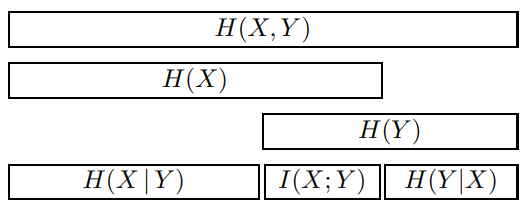
\includegraphics[width=0.7\textwidth]{images/mutua_info.png}
	\caption{Interpretazione grafica di entropia congiunta, condizionata e mutua informazione.}
\end{figure}

\textbf{Dimostrazione}:
$$
I(X;Y)=\sum_{x,y}P(x,y)\log\frac{P(x,y)}{P(x)P(y)}
=\sum_{x,y}P(x,y)\log\frac{P(x|y)P(y)}{P(x)P(y)} =
$$
$$
=\sum_{x,y}P(x,y)(\log P(x|y) + \log\frac{1}{P(x)}) 
=\sum_{x,y}P(x,y)\log\frac{1}{P(x)}+\sum_{x,y}P(x,y)\log P(x|y)
$$

la prima parte per il teorema delle probabilità totali è semplicemente:
$$
= H(x)+\sum_{x,y}P(x,y)\log P(x|y)= H(X)-\sum_{x,y}P(x,y)\log\frac{1}{P(x|y)} = H(X)-H(X|Y)
$$

\subsection{Proprietà della Mutua Informazione}
La Mutua Informazione comprende diverse proprietà:
\begin{enumerate}
	\item $I(X;X)=H(X)$ -- Dimostrazione: $H(X)-H(X|X)=H(X)$
	\item  $I(X;Y)=I(Y;X)$
	\item $I(X;Y)\ge 0$ -- Dimostrazione:\\ $$\sum_{x\in A_X}\sum_{y\in A_Y}P(x,y)\log_2\frac{P(x,y)}{P(x)P(y)}$$ poniamo: 
	$$
	\widehat{P}(x,y) = P(x,y) \quad \text{e} \quad \widehat{Q}(x,y) = P(x)P(y)
	$$
	
	e applichiamo la Diseguaglianza di Gibbs.
\end{enumerate}


\newpage

\subsubsection{Esempio N.4 - Mutua Informazione}
Supponiamo di avere le seguenti variabili aleatorie $X$ e $Y$ definite in $A=\{1, 2\}$ e con le seguenti probabilità note:\\
\begin{minipage}{0.50\textwidth}
	\begin{center}
		$$
		Pr[x=1 \wedge y=1] = 0
		$$
		$$
		Pr[x=2 \wedge y=1] = \frac{3}{4}
		$$
	\end{center}
\end{minipage}
\begin{minipage}{0.50\textwidth}
	\begin{center}
		$$
		Pr[x=1 \wedge y=2] = \frac{1}{8}
		$$
		$$
		Pr[x=2 \wedge y=2] = \frac{1}{8}
		$$
	\end{center}
\end{minipage}

Calcolare la Mutua Informazione $I(X;Y)$

Per calcolare $I(X;Y)$ devo prima calcolare $H(X)$ e $H(X|Y)$.\\ Per $H(X)$ devo calcolare $Pr(x)$ che, per il Teorema della Probabilità Totale, diventa:
$$
Pr(x) = \sum_{y} Pr[x \wedge y] = Pr[x \wedge y=1] + Pr[x \wedge y=2]
$$
Lo divido nei casi $x=1$ e $x=2$:
\begin{enumerate}
	\item $Pr[x=1] = Pr[x=1 \wedge y=1] + Pr[x=1 \wedge y=2] = 0 + \frac{1}{8} = \frac{1}{8}$
	\item $Pr[x=2] = Pr[x=2 \wedge y=1] + Pr[x=2 \wedge y=2] = 
	\frac{3}{4} + \frac{1}{8} = \frac{7}{8}$
\end{enumerate}

Adesso posso trovare $H(X)$:
$$
H(X) = \frac{1}{8}\ \log_{2}8 + \frac{7}{8}\ \log_{2} \frac{8}{7} \approx 0,375 + 0,169 = 0,544
$$
Per trovare $H(X|Y)$ calcolo prima $H(X|Y=1)$ e $H(X|Y=2)$ per poi calcolare:
$$
H(X|Y) = Pr[Y=1]\cdot H(X|Y=1) + Pr[Y=2]\cdot H(X|Y=2)
$$
So che $H(X|Y=1)$ equivale a:
$$
H(X|Y=1) = \sum_{x}\ Pr[X=x|Y=1] \log_{2} \frac{1}{Pr[X=x|Y=1]} = 
$$
$$
= Pr[x=1|y=1] \log_{2} \frac{1}{Pr[x=1|y=1]} + Pr[x=2|y=1] \log_{2} \frac{1}{Pr[x=2|y=1]} =
$$

Per il teorema della Probabilità Condizionata:\\
\begin{minipage}{0.50\textwidth}
	\begin{center}
		$$
		Pr[x=1|y=1] = \frac{Pr[x=1 \wedge y=1]}{Pr[y=1]} = 0
		$$
	\end{center}
\end{minipage}
\begin{minipage}{0.50\textwidth}
	\begin{center}
		$$
		Pr[x=2|y=1] = \frac{Pr[x=2 \wedge y=1]}{Pr[y=1]} = 1
		$$
	\end{center}
\end{minipage}
$$
H(X|Y=1) =  0 + 0 = 0
$$

Applico lo stesso ragionamento per $H(X|Y=2)$:
$$
H(X|Y=2) = Pr[x=1|y=2] \log_{2} \frac{1}{Pr[x=1|y=2]} + Pr[x=2|y=2] \log_{2} \frac{1}{Pr[x=2|y=2]}
$$

Calcolo $P[y=2]$:
$$
Pr[y=2] = Pr[y=2 \wedge x=1] + Pr[y=2 \wedge x=2] = \frac{1}{8} + \frac{1}{8} = \frac{1}{4} 
$$

Per il teorema della Probabilità Condizionata:\\
\begin{minipage}{0.50\textwidth}
	\begin{center}
		$$
		Pr[x=1|y=2] = \frac{Pr[x=1 \wedge y=2]}{Pr[y=2]} = \frac{1}{8} \cdot 4 = \frac{1}{2}
		$$
	\end{center}
\end{minipage}
\qquad
\begin{minipage}{0.50\textwidth}
	\begin{center}
		$$
		Pr[x=2|y=2] = \frac{Pr[x=2 \wedge y=2]}{Pr[y=2]} = \frac{1}{8} \cdot 4 = \frac{1}{2}
		$$
	\end{center}
\end{minipage}
$$
H(X|Y = 2) = \frac{1}{2}\cdot \log_{2} 2 + \frac{1}{2}\cdot \log_{2} 2 = 1
$$
Quindi $H(X|Y)$ equivale a:
$$
H(X|Y) = Pr[Y=1] \cdot 0 + \frac{1}{4} \cdot 1 = \frac{1}{4}
$$

Possiamo infine calcolare $I(X;Y) = H(X) - H(X|Y) = 0,544 - 0,150 = 0,394$


